\documentclass[11pt]{article}

\usepackage{fancyhdr}
\usepackage{hyperref}
\usepackage{graphicx}
\usepackage{enumerate}
\usepackage[greek,dutch]{babel} 
\usepackage{listings}
\usepackage{color}
\usepackage{framed}
\usepackage{subfig}

\usepackage[applemac]{inputenc}
\usepackage[T1]{fontenc}
\usepackage[section]{placeins}

\pagestyle{fancy}


\definecolor{mygreen}{rgb}{0,0.6,0}
\definecolor{mygray}{rgb}{0.5,0.5,0.5}
\definecolor{mymauve}{rgb}{0.58,0,0.82}

\lstset{ %
  backgroundcolor=\color{white},         % size of fonts used for the code
  breaklines=true,                 % automatic line breaking only at whitespace
  captionpos=b,                    % sets the caption-position to bottom
  commentstyle=\color{mygreen},    % comment style
  escapeinside={\%*}{*)},          % if you want to add LaTeX within your code
  keywordstyle=\color{blue},       % keyword style
  stringstyle=\color{mymauve},     % string literal style
}



\interfootnotelinepenalty=10000


\title{Raport Project Databases Maart}
\author{Mathias Beke, Bruno Van de Velde, Elias Van Langenhove, Alexander Vanhulle, Timo Truyts}

\author{
  Mathias Beke
  \and
  Bruno Van de Velde
  \and
  Elias Van Langenhove
  \and
  Alexander Vanhulle
  \and
  Timo Truyts
}


\date{\today}


\setlength{\parindent}{0cm}

\begin{document}

\lhead{Raport Project Databases: Maart}
\rhead{}



\maketitle


\tableofcontents





\section{Status}




\subsection{Taakverdeling}


\begin{enumerate}
    
   \item todo    
    
\end{enumerate}




\section{Design}


\subsection{UML diagram}

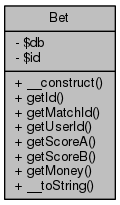
\includegraphics[scale=0.4]{UML_Bet.png}
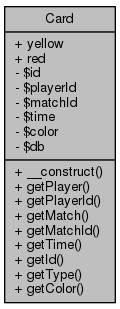
\includegraphics[scale=0.4]{UML_Card.png}
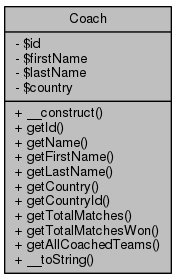
\includegraphics[scale=0.4]{UML_Coach.png}
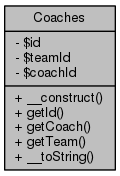
\includegraphics[scale=0.4]{UML_Coaches.png}
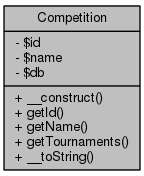
\includegraphics[scale=0.4]{UML_Competition.png}
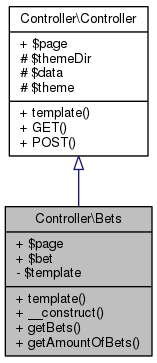
\includegraphics[scale=0.4]{UML_Controller_1_1Bets.png}
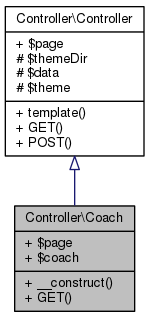
\includegraphics[scale=0.4]{UML_Controller_1_1Coach.png}
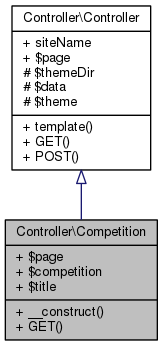
\includegraphics[scale=0.4]{UML_Controller_1_1Competition.png}
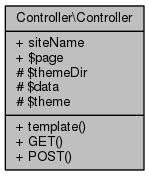
\includegraphics[scale=0.4]{UML_Controller_1_1Controller.png}
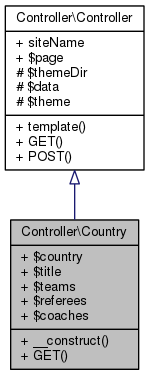
\includegraphics[scale=0.4]{UML_Controller_1_1Country.png}
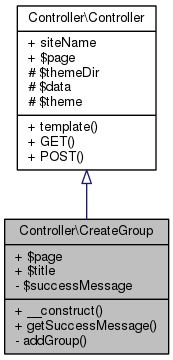
\includegraphics[scale=0.4]{UML_Controller_1_1CreateGroup.png}
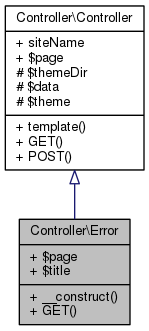
\includegraphics[scale=0.4]{UML_Controller_1_1Error.png}
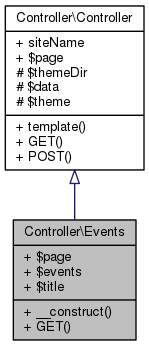
\includegraphics[scale=0.4]{UML_Controller_1_1Events.png}
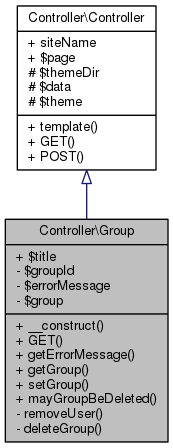
\includegraphics[scale=0.4]{UML_Controller_1_1Group.png}
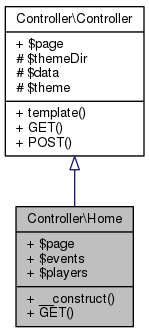
\includegraphics[scale=0.4]{UML_Controller_1_1Home.png}
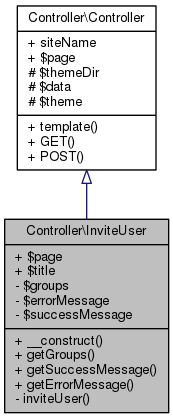
\includegraphics[scale=0.4]{UML_Controller_1_1InviteUser.png}
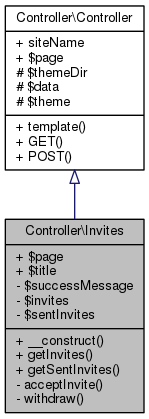
\includegraphics[scale=0.4]{UML_Controller_1_1Invites.png}
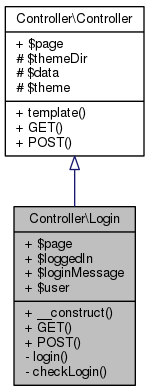
\includegraphics[scale=0.4]{UML_Controller_1_1Login.png}
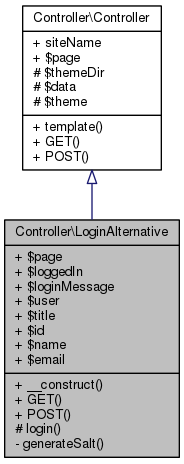
\includegraphics[scale=0.4]{UML_Controller_1_1LoginAlternative.png}
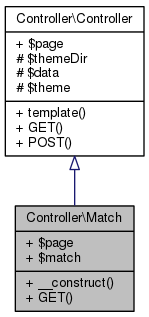
\includegraphics[scale=0.4]{UML_Controller_1_1Match.png}
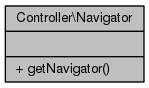
\includegraphics[scale=0.4]{UML_Controller_1_1Navigator.png}
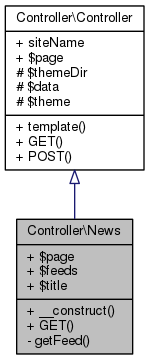
\includegraphics[scale=0.4]{UML_Controller_1_1News.png}
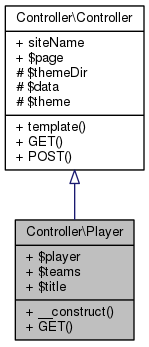
\includegraphics[scale=0.4]{UML_Controller_1_1Player.png}
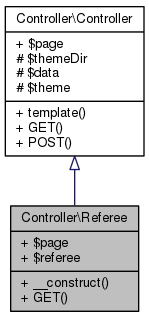
\includegraphics[scale=0.4]{UML_Controller_1_1Referee.png}
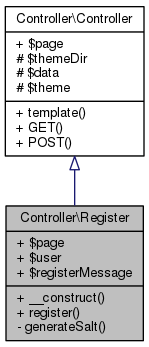
\includegraphics[scale=0.4]{UML_Controller_1_1Register.png}
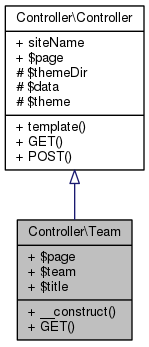
\includegraphics[scale=0.4]{UML_Controller_1_1Team.png}
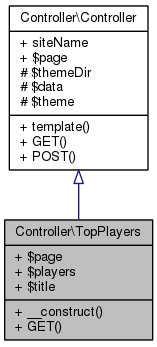
\includegraphics[scale=0.4]{UML_Controller_1_1TopPlayers.png}
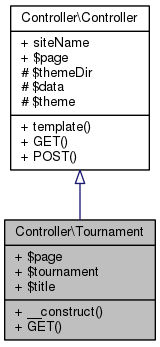
\includegraphics[scale=0.4]{UML_Controller_1_1Tournament.png}
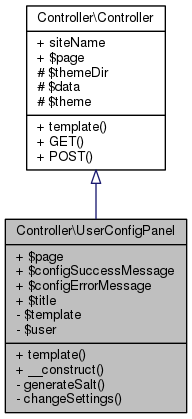
\includegraphics[scale=0.4]{UML_Controller_1_1UserConfigPanel.png}
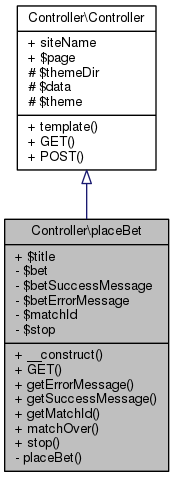
\includegraphics[scale=0.4]{UML_Controller_1_1placeBet.png}
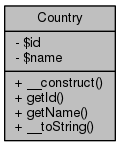
\includegraphics[scale=0.4]{UML_Country.png}
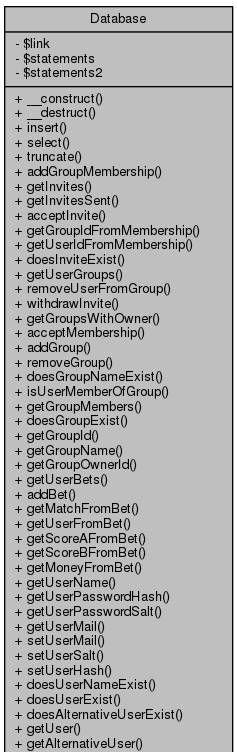
\includegraphics[scale=0.4]{UML_Database1.png}
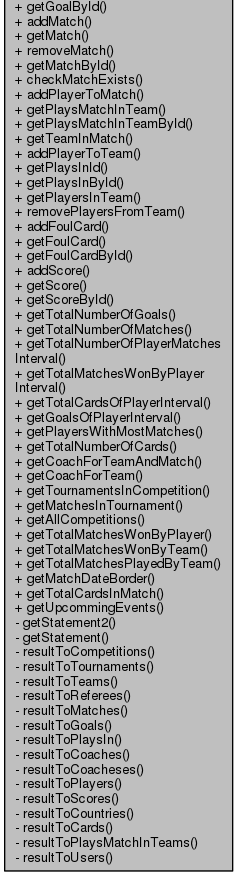
\includegraphics[scale=0.4]{UML_Database2.png}
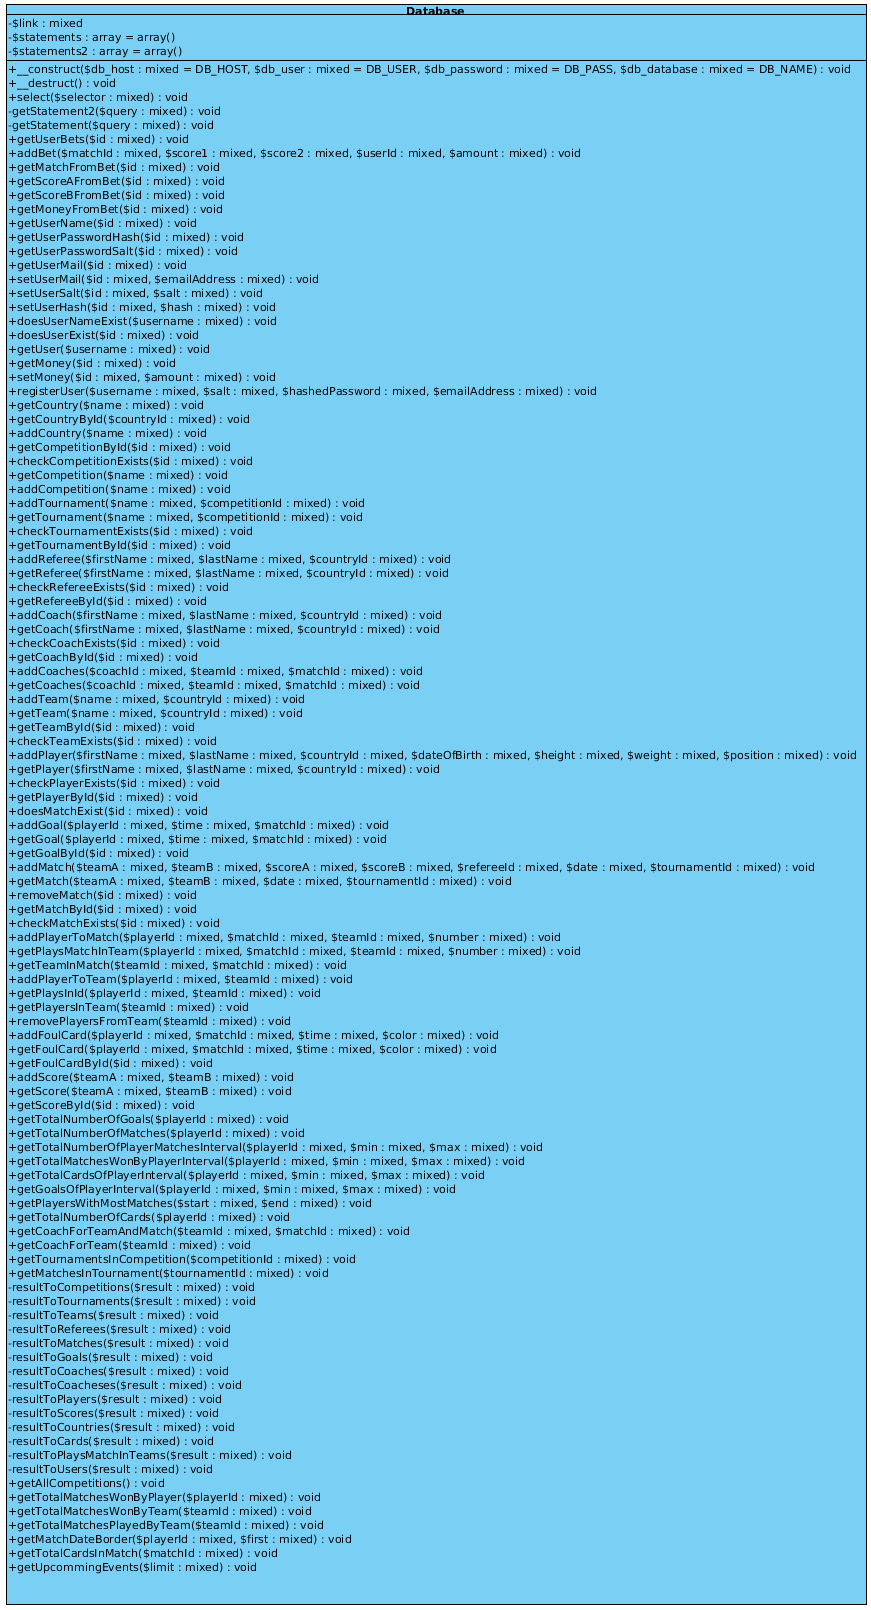
\includegraphics[scale=0.4]{UML_Database3.png}
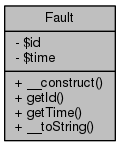
\includegraphics[scale=0.4]{UML_Fault.png}
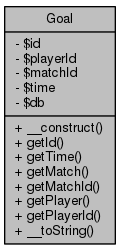
\includegraphics[scale=0.4]{UML_Goal.png}
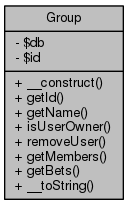
\includegraphics[scale=0.4]{UML_Group.png}
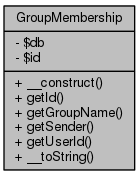
\includegraphics[scale=0.4]{UML_GroupMembership.png}
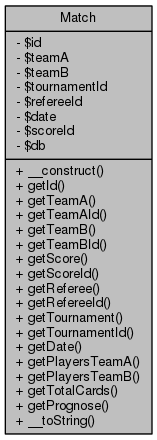
\includegraphics[scale=0.4]{UML_Match.png}
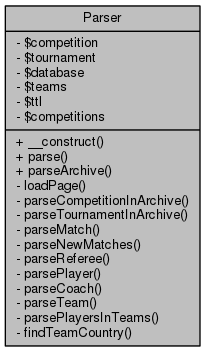
\includegraphics[scale=0.4]{UML_Parser.png}
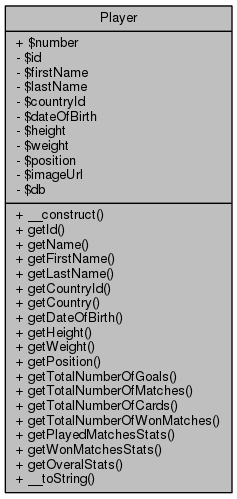
\includegraphics[scale=0.4]{UML_Player.png}
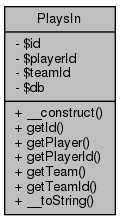
\includegraphics[scale=0.4]{UML_PlaysIn.png}
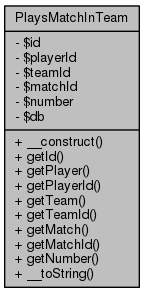
\includegraphics[scale=0.4]{UML_PlaysMatchInTeam.png}
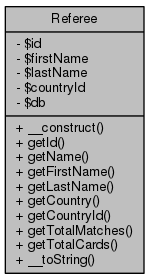
\includegraphics[scale=0.4]{UML_Referee.png}
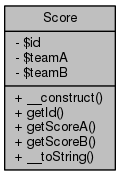
\includegraphics[scale=0.4]{UML_Score.png}
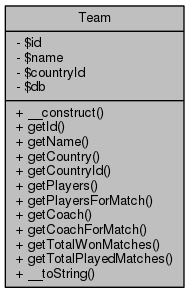
\includegraphics[scale=0.4]{UML_Team.png}
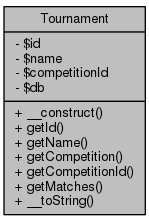
\includegraphics[scale=0.4]{UML_Tournament.png}
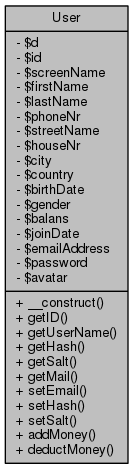
\includegraphics[scale=0.4]{UML_User.png}

\subsection{API}

Iemand?


\subsection{Parser (GO)}

Mathias




\section{Database}

\subsection{Schema (ERM-diagram)}

Alexander




\section{User Interface}


\subsection{Grafieken}

Timo







\subsection{Gebruikersgroepen}

Alexander



\section{Extra Functionaliteit}


\subsection{Wiki}

Elias



\subsection{RSS nieuwsfeed}

Mathias



\subsection{OpenID}

Naast de normale login is er ook een optie om in te loggen door gebruik te maken van een externe account. Wanneer je naar de alternatieve login pagina gaat, krijg je een keuze uit verschillende services (zoals Facebook en Google) waarmee je kunt inloggen. Buiten Facebook werken deze allen met openid en er is uiteindelijk voor de LightOpenID library gekozen omdat deze makkelijk te gebruiken was. Facebook is achteraf nog appart toegevoegd aangezien die helemaal geen OpenID provider is. Om in te kunnen loggen via Facebook moest eerst een app worden aangemaakt op hun site om alles mogelijk te maken. Buiten het feit dat er extra code nodig is die het verschil tussen een openid en een facebook login checked, is het grote nadeel dat de facebook login enkel op de server kan werken en niet ondertussen op de localhost getest kan worden. Maar dit heeft geen gevolgen voor de gebruikers van de site.




\section{Planning}


Iemand?



\section{Appendix}

\subsection{Queries}

Elias\\
Graag ook nu weer de code is zo'n box steken...


\paragraph{Gewonnen wedstrijden van speler binnen interval}

  Deze query vraagt de hoeveelheid matches waarbij de gegeven speler voor het winnende team speelde binnen een gegeven tijdspanne op.

  \begin{framed}
  \begin{lstlisting}[language=sql]
  SELECT COUNT(*)
   FROM `PlaysMatchInTeam`
   [JOIN `Match` ON `Match`.id = matchId]
   [JOIN `Score` ON `Score`.id = scoreId]
   [WHERE playerId = ? AND
   `Match`.date > ? AND
   `Match`.date < ? AND
      ((teamId = `Match`.teamA AND `Score`.teamA > `Score`.teamB) OR
      (teamID = `Match`.teamB AND `Score`.teamB > `Score`.teamA))];
  \end{lstlisting}
  \end{framed}



\end{document}
